\section{Testing Environment and Results}

The previous section described how the system was implemented and how each
component interacts within the complete flow, from a user that uploads a file to
the leader performing the Corruption Check phase (showed in Section
\ref{sec:check-corruption}).

This section presents the testing environment, the scenarios used during evaluation, and the obtained results. The tests were executed on a cluster of nine machines running Ubuntu 24.04.1 LTS (GNU/Linux 6.8.0-51-generic x86\_64). The specifications of the virtual machines are summarized in Table \ref{tab:vms-specs}. The nodes were geographically distributed across the European continent.

\begin{table}[h!]
    \centering
    \begin{tabular}{|l|c|c|c|c|c|}
    \hline
        \textbf{Node ID} & \textbf{IPv4} & \textbf{Country} & \textbf{CPU(s)} & \textbf{RAM} & \textbf{Disk} \\
       \hline
        GW & 51.15.221.121 & France & 8 & 32 GB & 45 GB \\
        Agent 1 & 212.47.241.22 & France & 4 & 16 GB & 45 GB \\
        Agent 2 & 51.15.138.169 & France & 4 & 16 GB & 45 GB \\
        Agent 3 & 51.159.178.75 & France & 4 & 8 GB & 45 GB \\
        Agent 4 & 51.158.75.32 & France & 4 & 8 GB & 45 GB \\
        Agent 5 & 51.158.233.202 & Netherlands & 4 & 8 GB & 45 GB \\
        Agent 6 & 51.15.108.2 & Netherlands & 4 & 8 GB & 45 GB \\
        Agent 7 & 151.115.42.176 & Poland & 4 & 8 GB & 45 GB \\
        Agent 8 & 151.115.104.48 & Poland & 4 & 8 GB & 45 GB \\
        \hline
    \end{tabular}
    \caption{Specifications of the machines used in the testing environment.}
    \label{tab:vms-specs}
\end{table}

Each test scenario considered four parameters:
\begin{itemize}
    \item \textbf{Number of agents}: total number of agents participating in the Reed-Solomon configuration of $n + k$ nodes.
    \item \textbf{Number of offline agents}: number of agents intentionally
        disconnected during the corruption check.
    \item \textbf{Number of files}: number of files included in the test.
    \item \textbf{File size}: size of each uploaded file. In the first four tests, each file is divided into $n + k$ shards, so the size of a single shard equals $\frac{\text{file size}}{\text{number of agents}}$.
\end{itemize}

All scenarios consider that some agents, respecting the Reed-Solomon requirement, could be offline during the uploads. In these scenarios, the time required for shard recovery, as described in Section \ref{sec:recovery-of-missing-shards}, is included in the measurement. The corruption check procedure begins only after all shards have been successfully uploaded to the cluster. The total elapsed time, measured in seconds, is recorded from the initiation of the corruption check until its completion. A test is considered valid only if the system successfully detects any data corruption. Each plotted value represents the average total elapsed time over three independent runs.

\paragraph{Test 1: Large files, all agents online}

In the first scenario, 100 files of 100 MB each were uploaded, yielding a total
dataset of 10 GB. Each file was divided into $n+k$ shards and distributed across
the agents in the cluster. All agents remained online during the corruption
check. Figure \ref{fig:test-1} shows the elapsed time for the corruption check
as the number of agents increases from 3 to 8. 
As expected, the elapsed time increases with the number of agents, primarily due
to additional network communication, coordination, and data verification
overhead. The elapsed time ranges from 1.373 seconds with 3 agents to 23.892 seconds with 8 agents.

\begin{figure}[!ht]
\centering
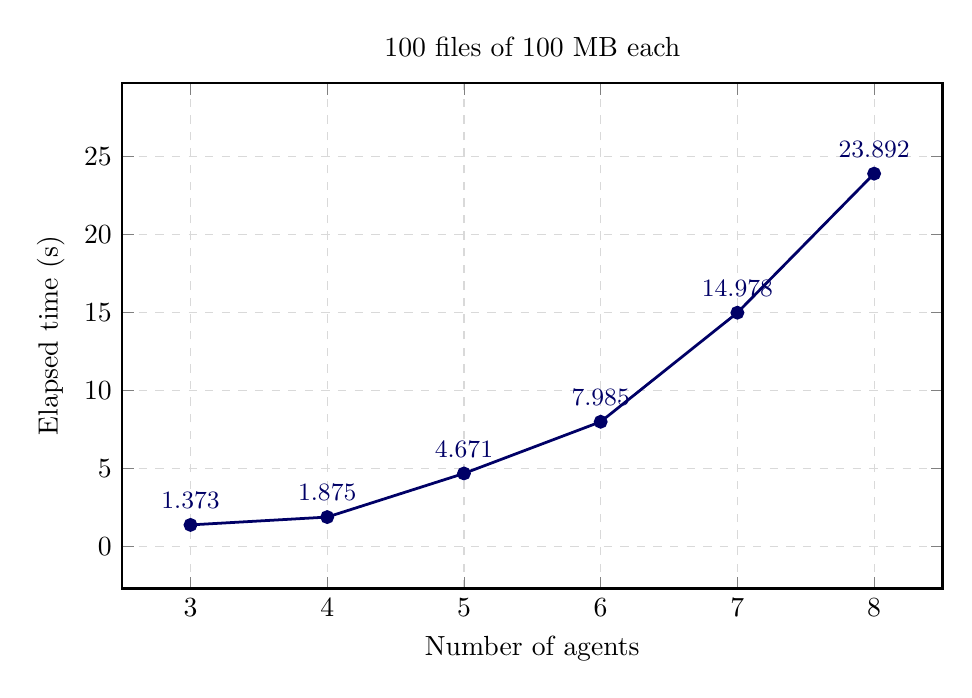
\begin{tikzpicture}
\begin{axis}[
    width=12cm, height=8cm,
    xlabel={Number of agents},
    ylabel={Elapsed time (s)},
    xmin=3, xmax=8,
    ymin=0, ymax=27,
    xtick={3,4,5,6,7,8},
    ytick={0,5,10,15,20,25},
    grid=major,
    grid style={dashed,gray!30},
    thick,
    title={100 files of 100 MB each},
    enlargelimits=0.1,
    clip=false,
    nodes near coords,
    every node near coord/.append style={font=\small, anchor=south, yshift=2pt},
    point meta=explicit symbolic
]

\addplot[color=blue!40!black, mark=*, line width=1pt] coordinates {
    (3,1.373) [1.373]
    (4,1.875) [1.875]
    (5,4.671) [4.671]
    (6,7.985) [7.985]
    (7,14.978) [14.978]
    (8,23.892) [23.892]
};
\end{axis}
\end{tikzpicture}
\caption{Elapsed time for the corruption check with 100 files of 100 MB each,
    with all agents online. Each agent stores 100 $\times$ (100 MB / number of agents) of data.}
\label{fig:test-1}
\end{figure}


\newpage
\paragraph{Test 2: Many small files, all agents online}

The second test involved 10,000 files of 1 MB each, maintaining the same total
dataset size of 10 GB. This scenario highlights the impact of a high file count
relative to file size. As shown in Figure \ref{fig:test-2}, elapsed time
increases substantially with the number of agents, from 0.469 seconds with 3
agents to 81.032 seconds with 8 agents. The growth compared to Test 1
indicates that the number of files significantly influences corruption check
performance, primarily due to the overhead of managing numerous small shards.

\begin{figure}[!ht]
\centering
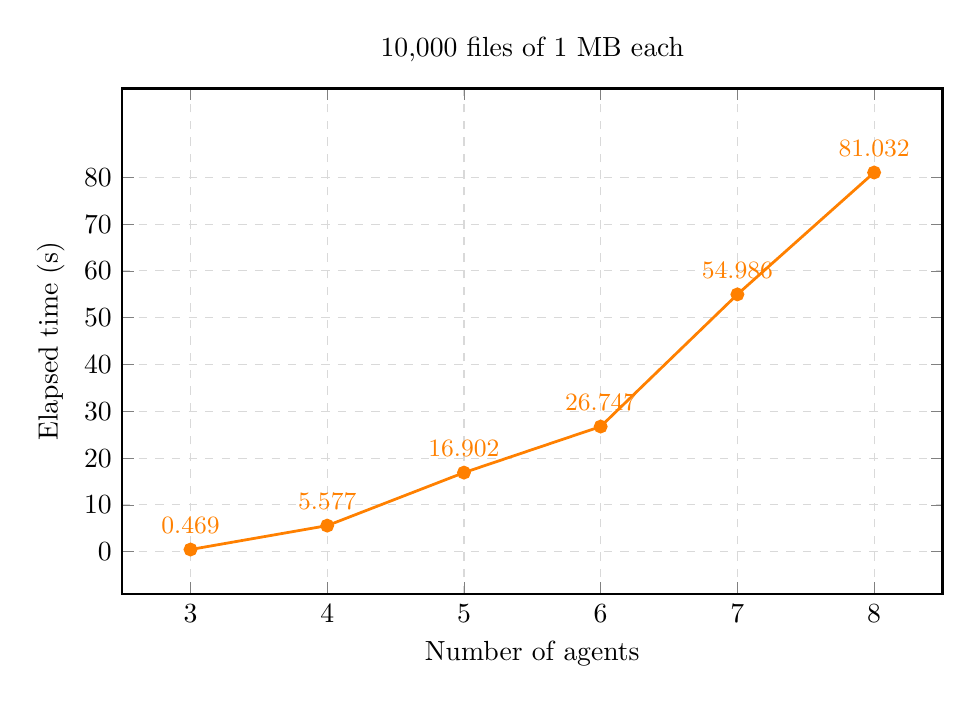
\begin{tikzpicture}
\begin{axis}[
    width=12cm, height=8cm,
    xlabel={Number of agents},
    ylabel={Elapsed time (s)},
    xmin=3, xmax=8,
    ymin=0, ymax=90,
    xtick={3,4,5,6,7,8},
    ytick={0,10,20,30,40,50,60,70,80},
    grid=major,
    grid style={dashed,gray!30},
    thick,
    title={10,000 files of 1 MB each},
    enlargelimits=0.1,
    clip=false,
    nodes near coords,
    every node near coord/.append style={font=\small, anchor=south, yshift=2pt},
    point meta=explicit symbolic
]

\addplot[color=orange, mark=*, line width=1pt] coordinates {
    (3,0.4685) [0.469]
    (4,5.577) [5.577]
    (5,16.902) [16.902]
    (6,26.747) [26.747]
    (7,54.986) [54.986]
    (8,81.032) [81.032]
};
\end{axis}
\end{tikzpicture}
\caption{Elapsed time for the corruption check with 10,000 files of 1 MB each,
    with all agents online. Each agent stores 10,000 $\times$ (1 MB / number of agents) of data.}
\label{fig:test-2}
\end{figure}

\newpage
\paragraph{Test 3: Large files, but small dataset}

This test evaluates system performance on a small dataset consisting of 10 files, each 1 GB in size, under different cluster sizes. All agents remained online during the corruption check. Figure \ref{fig:test-3} shows the elapsed time as the number of agents increases from 3 to 8. As expected, the elapsed time grows with the number of agents, mainly due to increased network communication overhead and coordination between nodes.

Interestingly, even though the total dataset size (10 GB) is comparable to
Tests 1 and 2, the overall elapsed time is significantly lower. This suggests
that the system handles a smaller number of large files more efficiently than
many smaller files. This behavior could indicate that the corruption check mechanism scales better with file size than with file count.

\begin{figure}[!ht]
\centering
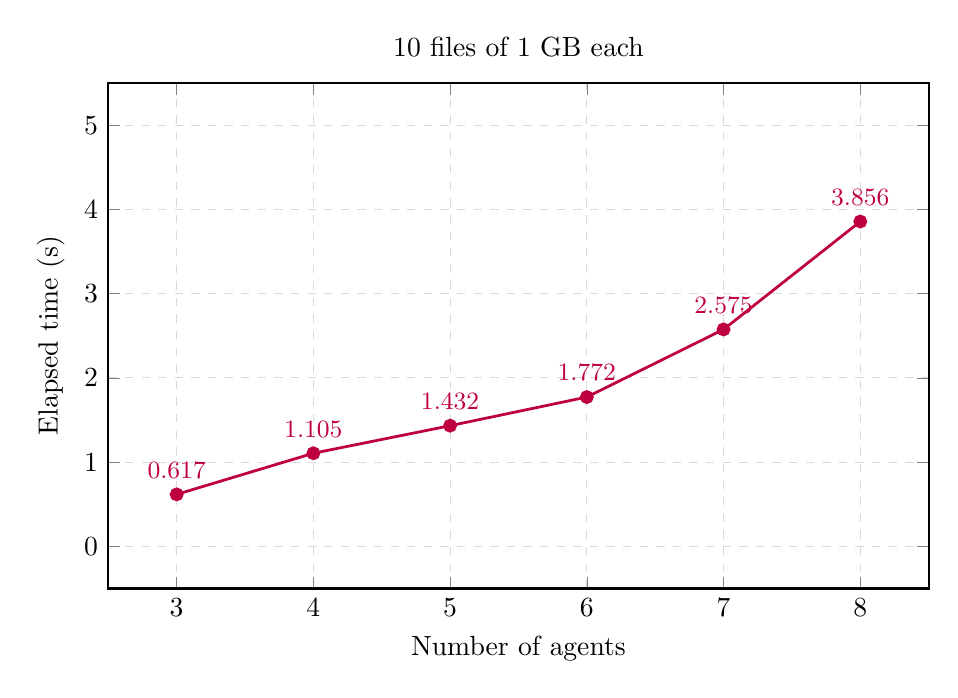
\begin{tikzpicture}
\begin{axis}[
    width=12cm, height=8cm,
    xlabel={Number of agents},
    ylabel={Elapsed time (s)},
    xmin=3, xmax=8,
    ymin=0, ymax=5,
    xtick={3,4,5,6,7,8},
    ytick={0,1,2,3,4,5},
    grid=major,
    grid style={dashed,gray!30},
    thick,
    title={10 files of 1 GB each},
    enlargelimits=0.1,
    clip=false,
    nodes near coords,
    every node near coord/.append style={font=\small, anchor=south, yshift=2pt},
    point meta=explicit symbolic
]

\addplot[color=purple, mark=*, line width=1pt] coordinates {
    (3,0.6166) [0.617]
    (4,1.105) [1.105]
    (5,1.432) [1.432]
    (6,1.772) [1.772]
    (7,2.575) [2.575]
    (8,3.856) [3.856]
};
\end{axis}
\end{tikzpicture}
\caption{Elapsed time for the corruption check with 10 files of 1 GB each, with all agents online. Each agent stores $10 \times (1 \text{ GB} / \text{number of agents})$ of data.}
\label{fig:test-3}
\end{figure}
\newpage
\paragraph{Test 4: Small files, partially offline agents}

The fourth scenario evaluates the effect of offline agents. 1,000 files of 150 KB
each were uploaded, and elapsed time was measured both with all agents online
and with a subset of agents offline during the corruption check.
Figure \ref{fig:test-4} compares the two configurations. Offline agents
introduce additional latency due to the timeout before retrieving the previous
saved hash, with elapsed times ranging from 28.2 to 91.338 seconds, compared to 3.1 to 69.221 seconds when all agents are online.

\begin{figure}[!ht]
\centering
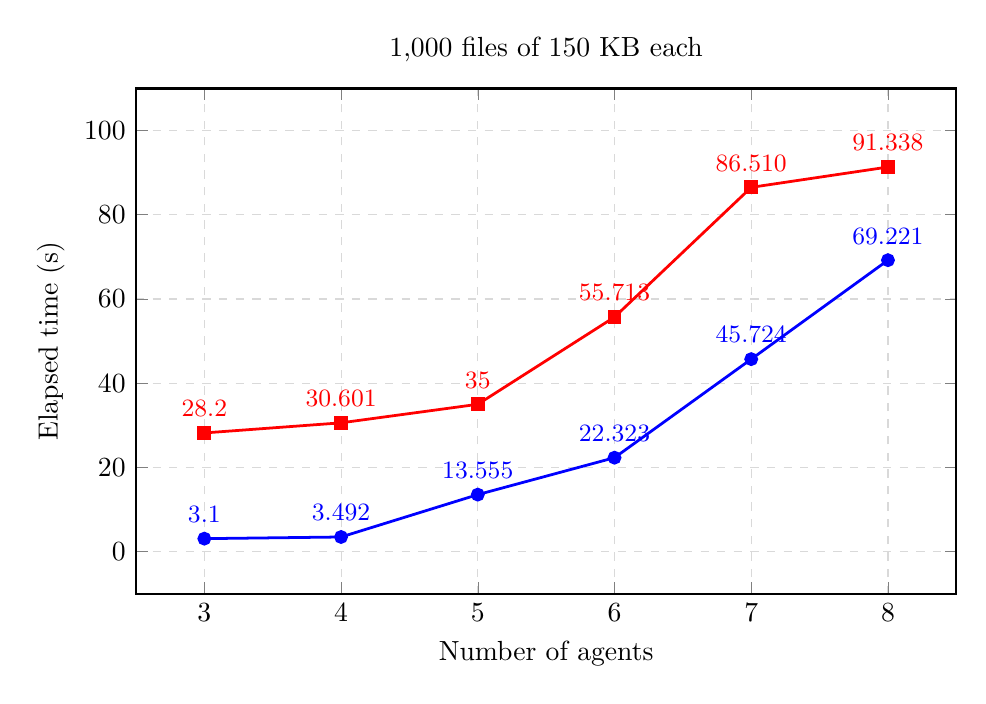
\begin{tikzpicture}
\begin{axis}[
    width=12cm, height=8cm,
    xlabel={Number of agents},
    ylabel={Elapsed time (s)},
    xmin=3, xmax=8,
    ymin=0, ymax=100,
    xtick={3,4,5,6,7,8},
    ytick={0,20,40,60,80,100},
    grid=major,
    grid style={dashed,gray!30},
    thick,
    title={1,000 files of 150 KB each},
    enlargelimits=0.1,
    clip=false,
    nodes near coords,
    every node near coord/.append style={font=\small, anchor=south, yshift=2pt},
    point meta=explicit symbolic
]

% Online agents
\addplot[color=blue, mark=*, line width=1pt] coordinates {
    (3,3.1) [3.1]
    (4,3.492) [3.492]
    (5,13.555) [13.555]
    (6,22.323) [22.323]
    (7,45.724) [45.724]
    (8,69.221) [69.221]
};

% Offline agents
\addplot[color=red, mark=square*, line width=1pt] coordinates {
    (3,28.2) [28.2]
    (4,30.601) [30.601]
    (5,35) [35]
    (6,55.713) [55.713]
    (7,86.510) [86.510]
    (8,91.338) [91.338]
};

\end{axis}
\end{tikzpicture}
\caption{Elapsed time of the corruption check with 1,000 files, each 150 KB in
    size. Each agent stores 1,000 $\times$ (150 KB / number of agents) of data. In blue with none offline agents; in red with offline
    agents.}
\label{fig:test-4}
\end{figure}

\newpage
\paragraph{Test 5: Very large number of tiny files}

The last test evaluates system performance with an extremely large number of very small files. The dataset consisted of one million files, distributed across different cluster configurations. Unlike the previous tests, where file sizes varied with the number of agents, in this case each file had a fixed size of 4 KB. Consequently, increasing the number of agents also increases the total global dataset size, allowing an assessment of how the system handles both a high file count and a growing overall workload.

Figure \ref{fig:test-5} shows the total elapsed time for the corruption check as
the number of agents increases. Despite the large file count, the system
maintains acceptable performance, with time increasing gradually as more agents
participate. This behavior highlights the scalability of the corruption check
mechanism, which efficiently verifies tasks across nodes. However, the absolute
elapsed time is significantly higher than in previous tests with fewer, larger
files, reinforcing that per-file management overhead dominates when processing
millions of small files. The test demonstrates that while the system remains
operationally robust, optimizing metadata handling and batching operations could
further improve scalability for dataset dominated by small files.

\begin{figure}[!ht]
\centering
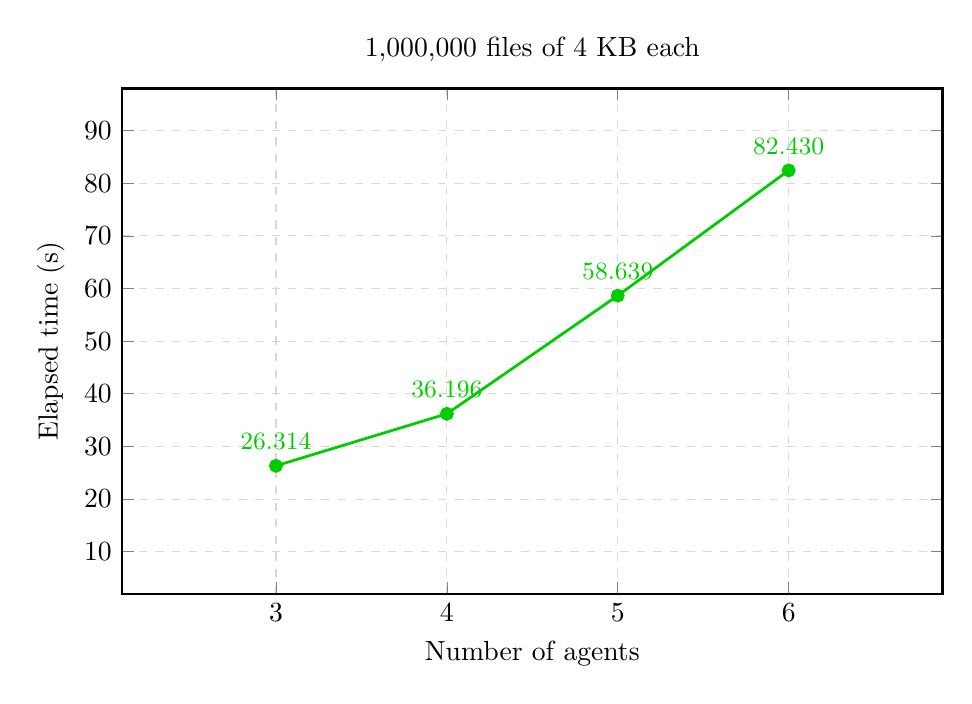
\begin{tikzpicture}
\begin{axis}[
    width=12cm, height=8cm,
    xlabel={Number of agents},
    ylabel={Elapsed time (s)},
    xmin=2.5, xmax=6.5,
    ymin=10, ymax=90,
    xtick={3,4,5,6},
    ytick={0,10,20,30,40,50,60,70,80,90,100},
    grid=major,
    grid style={dashed,gray!30},
    thick,
    title={1,000,000 files of 4 KB each},
    enlargelimits=0.1,
    clip=false,
    nodes near coords,
    every node near coord/.append style={font=\small, anchor=south, yshift=2pt},
    point meta=explicit symbolic
]

\addplot[color=green!80!black, mark=*, line width=1pt] coordinates {
    (3,26.314) [26.314]
    (4,36.196) [36.196]
    (5,58.639) [58.639]
    (6,82.430) [82.430]
};
\end{axis}
\end{tikzpicture}
\caption{Elapsed time for corruption check on very large datasets. The total dataset size increases
    with the number of agents: 12 GB for 3 agents, 16 GB for 4 agents, 20 GB
    for 5 agents, and 24 GB for 6 agents. Each agent stores 4 GB of data.}
\label{fig:test-5}
\end{figure}

\newpage

\paragraph{Results}

The experimental evaluation demonstrates that the system maintains correctness and functional reliability across a wide variety of scenarios. However, performance degrades as the cluster size increases, primarily due to the coordination and communication overhead introduced by the Raft consensus, as well as the computational cost of Merkle tree operations and network latency when retrieving root hashes from agents.

In Test 1, with 100 files of 100 MB each (10 GB total), the elapsed time
increased from 1.37 seconds with 3 agents to 23.89 seconds with 8 agents. This trend shows that the system remains functional but becomes progressively slower as coordination overhead grows.

In Test 2, using 10,000 files of 1 MB each (10 GB total), elapsed time increased
from 0.47 seconds with 3 agents to 81.03 seconds with 8 agents. This represents about
170x increase, clearly showing that scenarios with many small files amplify the cost of synchronization and consensus, leading to diminishing performance returns as the cluster expands.

Test 3, with 10 files of 1 GB each (10 GB total), exhibited a milder increase
(from 0.62 seconds to 3.86 seconds) indicating that the system handles large files more efficiently. Compared to Tests 1 and 2, this suggests that performance loss is primarily driven by the number of files (and resulting coordination steps), not by total data size.

In Test 4, with 1,000 files of 150 KB each (150 MB total), the system was evaluated under partial node unavailability. When some agents were offline, execution time increased by roughly 9x (for example, from 3.1 seconds to 28.2 seconds with 3 agents). However, the relative slowdown diminished with larger clusters, confirming that Raft's fault-tolerant synchronization mitigates the effects of offline nodes, albeit at a cost in latency.

Finally, Test 5, involving one million files of 4 KB each, measured total
processing time from 26.31 seconds to 82.43 seconds as dataset size grew from 12 GB to 24
GB. Despite the large number of files, absolute latency grows and the system continues to process data at a predictable rate.

Overall, the results show that the system is robust but not
performance-scalable. It preserves data integrity and correctness under varying
dataset and node conditions, but verification time increases disproportionately
with the number of agents and files. These findings highlight the trade-off
between distributed consistency and performance in consensus-based integrity
verification protocols.
